
\chapterimage{chapter_head_4.jpg} % Chapter heading image

\chapter{Facilities}
\addcontentsline{lof}{figure}{Chapter header \emph{Branches}: Photo credit to
Kira Liebert}
\addtocontents{lof}{\protect\vspace{\baselineskip}}
 
\section{New College}

\subsection{The MCR - The Rew Nooner Spoom}\label{ssec:Spoom}

This is your common room - the actual MCR. It was named after the Rev. Spooner, Warden of New College from 1903-1924, who was famous for his verbal gags or \emph{Spoonerisms}: hence the name. The MCR is commonly called \emph{the Spoom}. It is accessible 24 hours a day and has a 42'' television, Nintendo Wii, PS4 (doubling as BD/DVD-player), board games, books, coffee machine, wi-fi, and newspapers as well as other publications. The TV somes equiped with Netflix and a wide range of TV channels including Sky Movie, Sky Atlantic, Sky Sports, BT Spotrs and ESPN. It also has a bar area which is opened regularly - usually on Wednesday and Thursday nights during term time, as well as after guest night dinners. It is also used for other purposes, including a free brunch each Sunday morning during term time.

Since 2009, the Spoom has been located in the Weston Sports Pavilion.
Refurbished recently, the Rew Nooner Spoom (New Spooner Room) is undoubtedly one
of the most comfortable and inviting MCRs in Oxford. The facilities are split
across the main living room area upstairs and the television and computer room
downstairs, which also has a small library.
Access to these rooms and indeed the Sports Pavilion is since 2013 by your
bod-card. If you are confronted with any bod-card malfunction issues, contact
either Lauren Burton (\href{mailto:lauren.burton@new.ox.ac.uk}{\urlformat{lauren.burton@new.ox.ac.uk}}), or the deputy clerk of works, Chris Conway (\href{mailto:chris.conway@new.ox.ac.uk}{\urlformat{chris.conway@new.ox.ac.uk}}).

\begin{figure}[htbp]
\centering
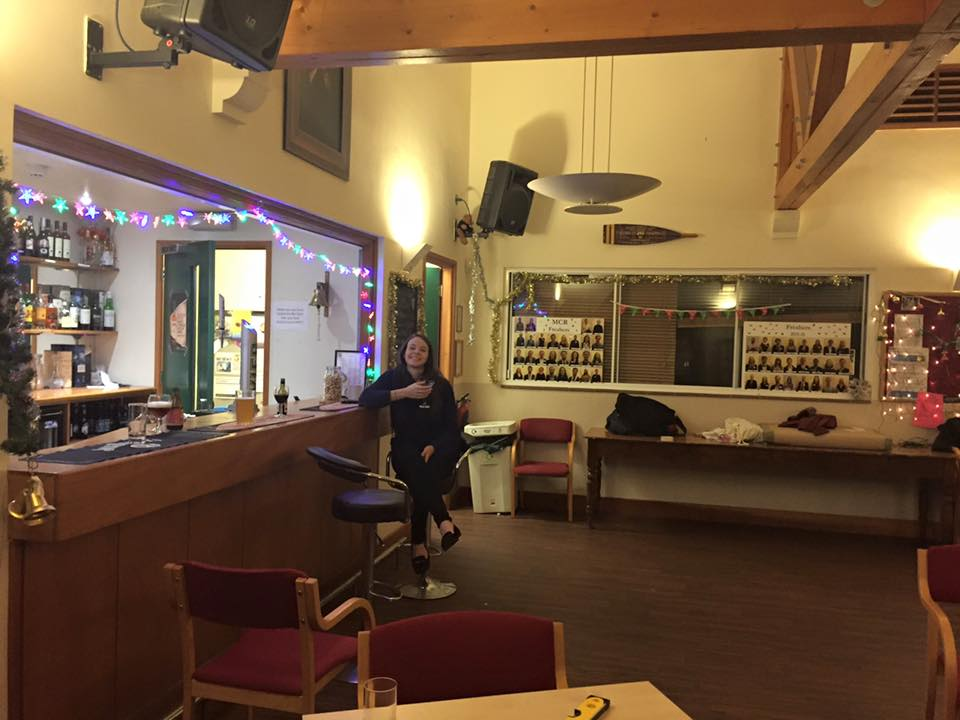
\includegraphics[width=0.85\textwidth]{Spoom.jpg}
\caption[]{The Rew Nooner Spoom}
\label{fig:Spoom}
\end{figure}

\subsection{The JCR}

Graduate students are also members of the Junior Common Room (primarily the undergraduate body of college). The physical JCR is located in the Garden Quad and has a satellite television, pool table and games consoles. There are also a few computers that can be access with New College credentials.
\subsection{Hall}

\emph{Hall} refers to the dining hall in college. The Hall is located in the oldest
part of college with the buttery next to it. Food is available to graduates during term time; all meals are charged to your till account and paid for using your Bod-card (see below). 

\smallskip

\begin{description}
\item[Breakfast:] Breakfast is available from 8\,am to 9\,am on weekdays
and 11\,am to 1\,pm at weekends. A choice of an \emph{English} cooked breakfast,
\emph{continental} breakfast, cereal etc. is available and charged per item, for
a total of about \pounds1.50-\pounds2.00.
\item[Lunch:] Lunch is available 12\,am to 1.30\,pm on weekdays. Lunch can be
charged per item individually, a meal consisting of main, potatoes, veg and
salad will be charged at \pounds3.50.
\item[Dinner:] 
Dinner comes in two sittings, early and late, usually referred to as \emph{informal
hall} and  \emph{formal hall} respectively. As of
October 2014, evening meals cost \pounds6.26 inclusive of soup, salads, a main
course, potatoes/pasta, vegetables, and dessert. Students MUST book their meals before
10\,am on the day they want to go to dinner in the Hall. This is done on-line at
\url{http://food.new.ox.ac.uk/}, where you also have to specify the sitting you
wish to attend.

Informal hall is available every day, canteen style, and food can be bought
between 5:45\,pm to 7:00\,pm (6:30\,pm on Fridays). 

Formal hall is held every Tuesday, Thursday and
Sunday during term time, and is served. For formal hall diners
have to be seated for 7.15\,pm, stand when the Fellows enter, then sit after
saying grace. Unusually for Oxford, we do not stand up when the Fellows leave
at the end of dinner. During these dinner we have to wear gowns, but can wear
them over casual clothing.

There are occasionally other dinners, in particular guest night dinners, which
are held fortnightly on odd-numbered term weeks. These guest dinners are a great
favourite of the MCR for their lavish 3-course catering and the customary
after-parties. One great perk of New College dinning is that MCR members may
bring up to 4~guests. Guest night dinners are charged at \pounds~15.55 per
person.

\item[Dining on high table:] Fresher graduates may dine at high table once
during their first year with the Tutor for Graduates (if they reply fast enough
to the invitation emails).
This will be advertised during term. You could also try and persuade your college adviser to invite you to dine at high table.
\end{description}

\subsection{College Bar}
The college bar, beer cellar, or JCR bar, is primarily college run. It is open
all day offering sandwiches, cakes, coffee and beverages and starts serving
alcohol from 6\,pm to 11\,pm during term, and often out of term as well. The bar
is located under the hall and has games such as table football.

Drinks are cheap (considerably cheaper than in town), and priced at the
level of the MCR bar. You can pay cash but it is slightly cheaper to use your Bod-card and charge it to your till account.

\subsection{Sports facilities}
New College has one of the best and most beautiful sports grounds in Oxford, located a five-minute walk from college on St. Cross Road. This has football and rugby pitches, a cricket pitch and nets, one hard tennis court and six grass courts and a volleyball court in the summer. There is a squash court and table-tennis table in the pavilion. Many of the facilities can be in the Weston lodge or using the online booking system. There is plenty of equipment in the Weston lodge for many of these sports for use by MCR members. 

College has sports teams in a wide range of sports: details will be available during freshers' fortnight. The collegiate nature of the university makes it very easy to get involved in sport whilst at Oxford.

Rowing is very popular in Oxford. College has a boathouse on the Isis and a very active boat club. There will be several novice boats run during Michaelmas, as well as opportunities for experienced rowers. Again, these will be advertised in freshers' fortnight.

We also have a punt shed located at the sports ground; punts may be taken out
from here during the summer. New College does not have its own gym. However,
members of college have free access to the university gym at the Iffley Road. To
access the Iffley Road gym, simply bring your Bod card to the gym's front desk
and inform the attendant of your college membership. You will be asked to fill
out some paperwork. Another work-out option is the University Club, which is
very close to New College on Mansfield Road, and of which all Oxford graduate
students are members. A year-round pass to the Club's gym may be purchased for
around \pounds60.

\begin{figure}[htbp]
\centering
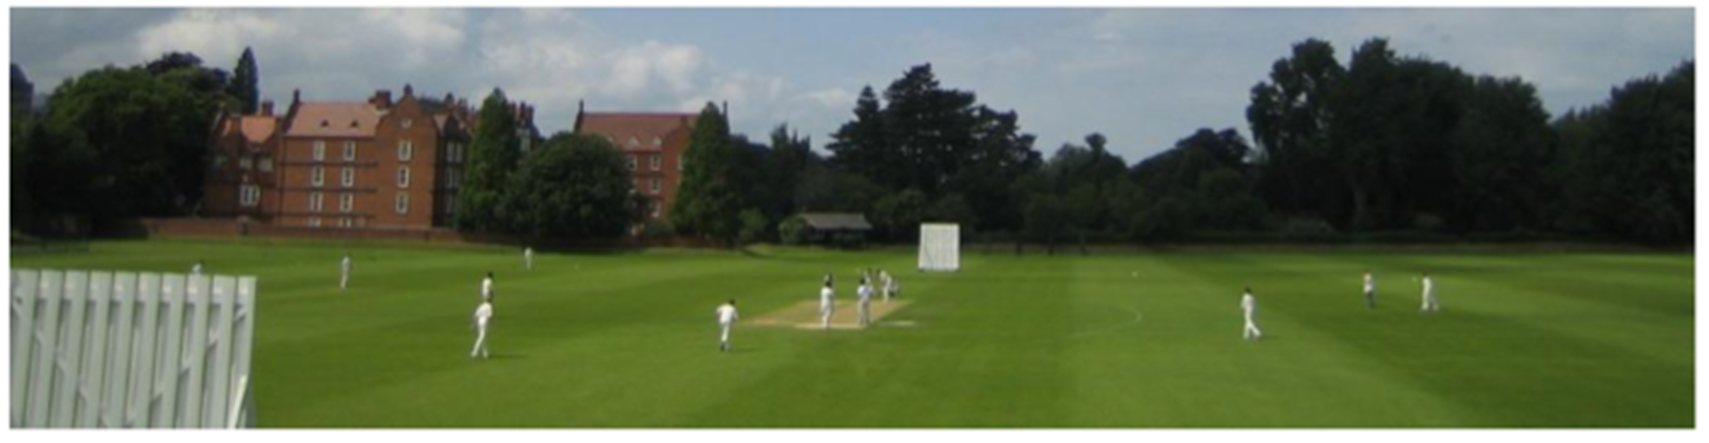
\includegraphics[width=0.9\textwidth]{sports.png}
\caption[]{The College sports ground}
\label{fig:sports}
\end{figure}

\subsection{MCR BBQ}
In 2013 we had a communal BBQ built behind the cricket pavilion overlooking the sports ground. It is currently available for MCR events only, but is intended to be accessible for any MCR member's private function in the future. The MCR committee usually organizes BBQ-related events in the end of Trinity term and during the summer break.
\subsection{The Library}
The College has a library which is located in the Holywell Quad. It is open from
8.30\,am to midnight during term and from 08.30-17.00 out of term (the student body is campaigning hard to lengthen these hours). The library's collection is aimed mainly at undergraduate studies; however, the library is also available for graduates to use for work. Books and DVDs may be borrowed from the College library.
\subsection{IT}
All rooms in college have ethernet access. This connection can be activated by plugging in your computer using an ethernet cable, opening your internet browser and following the automated security program. There is also wi-fi in the Spoom, Weston buildings, JCR and library which is activated in the same way. Returning students should  find that wi-fi coverage has now improved with reasonable signal reaching even the upstairs rooms. IT services are continually working to improve wireless internet connectivity throughout the college. 

There is an MCR computer room in the Sports Pavilion containing two PCs and a laser printer. There is also a JCR computer room in NB2, which has some more advanced printers. Printing is charged to your Battels. 

All college members will have a college e-mail address. Your address will be in the
form \emph{\nolinkurl{firstname.surname@new.ox.ac.uk}}. You will almost
certainly have a second one in your department but (with a few exceptions) they all go to the same account.
There will be details of how to set up your account in your pidge soon after you
arrive. There is a webmail interface, but the account is easy to configure for
an e-mail client. See: \url{http://www.oucs.ox.ac.uk/email/config/}

\subsection{Chapel}
The chapel welcomes all college members to its services, which take place during the eight weeks of university term. We hope the chapel will be a place where anyone can find community, inspiration in words and music, and calm during busy weeks. Services follow the pattern of the Anglican church: the music is sung by the chapel choir, which has an international reputation, and the liturgy is formal to fit in with the building and the music, but aims to be as inclusive as possible and to focus on issues in the wider world. Any college member is welcome to get involved in chapel life - as readers, servers, and chapel wardens.

Services are held every weekday evening apart from Wednesday. College communion is at 9\,am on Sunday and is followed by breakfast. Advent and Christmas Carol Services are held on the Sundays of 8th week and 9th week of Michaelmas Term.

The beautiful chapel is also close to the scenic cloisters, a favourite spot of many for its peaceful, shaded ambience. The scene in Harry Potter and the Goblet of Fire where Draco Malfoy is turned into a ferret was filmed in the cloisters here. 

All information about the chapel may be found on the termly chapel card copies
in pigeon holes and on the chapel and lodge notice boards and on the chapel page
of the college website, and the choir website (\url{www.newcollegechoir.com}).

\subsection{The Gardens}
New College has some beautiful gardens, which are the responsibility of the Garden Fellow, Robin Lane Fox. Nobody is permitted to walk on the grass in the Front Quad, but all other areas may be used by students. Croquet may be played in the Holywell Quad, but no other ball games are allowed.
The main gardens are surrounded by the city walls and contain a decorative
\emph{Mound}. Do not climb, or let your guests climb, the city walls: this is an
offence, not just at college, but also at university level and the punishment is to be sent down.

\subsection{Chalet}

During your time at New College, please take advantage of our chalet in the
French Alps. With Balliol College and University College, we share an historic
property near Mont Blanc, which in 2009 celebrated its 100th birthday following
its reconstruction after the original 1865 chalet was accidentally burnt down in
1906. Each summer, two or three groups from New College spend 10~days reading
and walking in one of the most beautiful parts of Europe. All members of the college are welcome.
Groups are normally a mix of undergraduates and postgraduates with a few members
of the SCR. The trip is very inexpensive (usually less than \pounds5 per day), and
travel by air through Geneva or on the sleeper train from Paris is easy. For
more information, please consult the college page on the chalet
(\url{http://www.new.ox.ac.uk/new-college-chalet}).

\begin{figure}[htbp]
\centering
		\begin{minipage}{0.3\textwidth}
                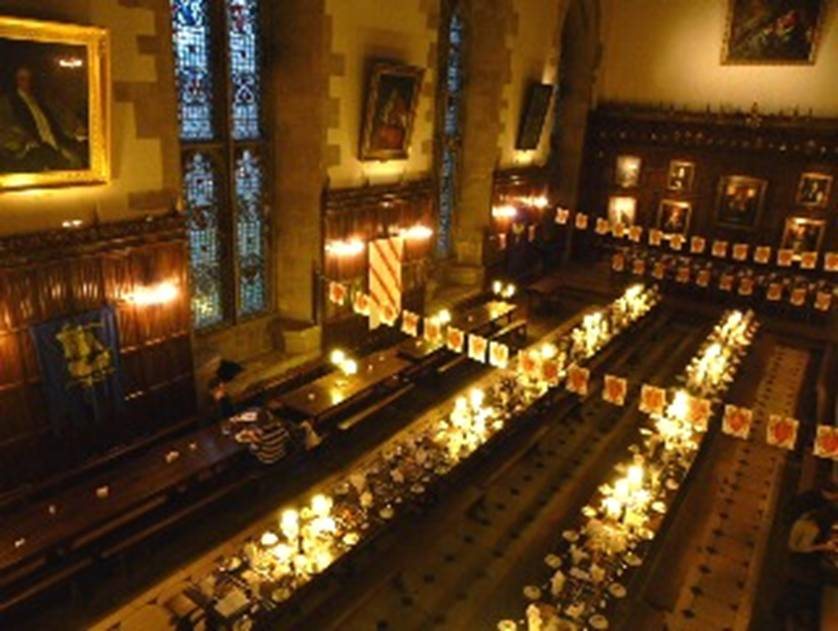
\includegraphics[width=\textwidth]{hall.jpg}
                \caption[Hall: Photo credit to Maureen Lenker]{The hall, set for
                a medieval dinner}
                \label{fig:hall}
        \end{minipage}%
        \quad
        \begin{minipage}{0.33\textwidth}
                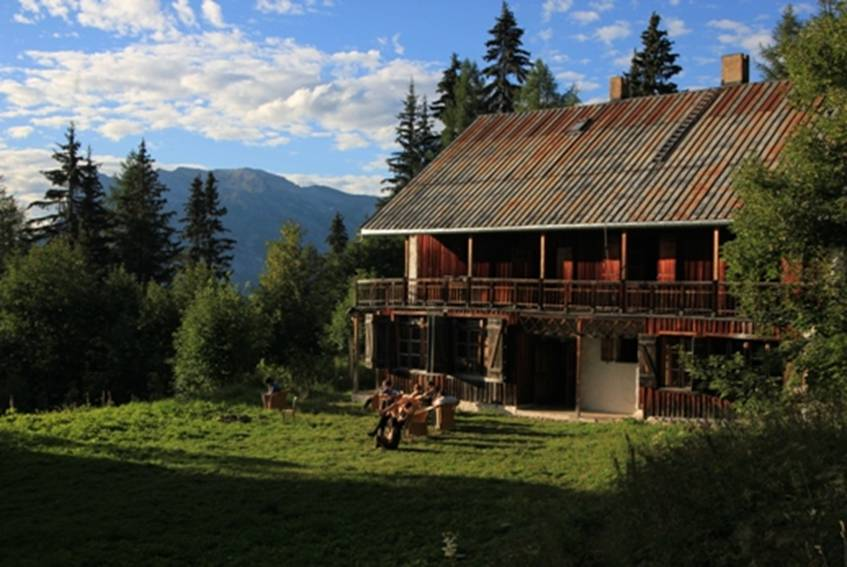
\includegraphics[width=\textwidth]{chalet.jpg}
                \caption[Chalet: Photo credit to Nick Altemose]{The
                \emph{cha\-let des ang\-lais}}
                \label{fig:chalet}
        \end{minipage}%
        \quad
        \begin{minipage}{0.3\textwidth}
                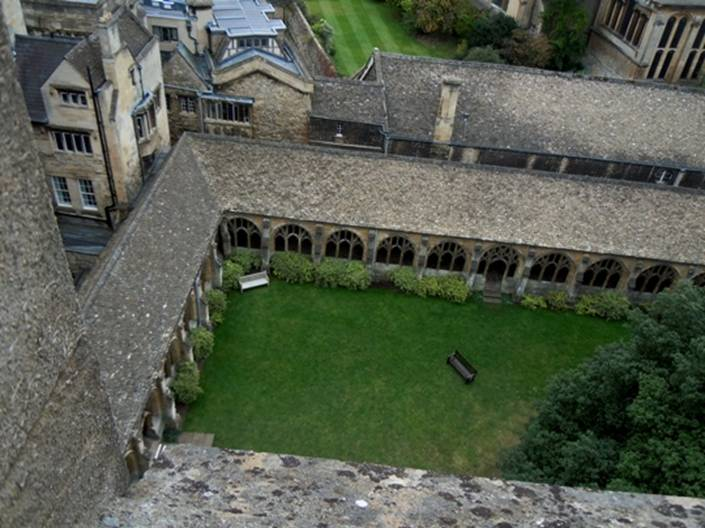
\includegraphics[width=\textwidth]{clois.jpg}
                \caption[Cloisters: Photo credit to Alex Graham]{The cloisters
                from New College tower}
                \label{fig:clois}
        \end{minipage}%
\end{figure}

\subsection{Pigeon hole}

You will be given a pigeon hole, referred to as your \emph{pidge}, in the post
room by the porters' lodge. This is where you collect your mail, both internal and external. Your address will be: Yourname,~New College,~Holywell~Street,~Oxford,~OX1~3BN,~UK.

You can send post internally across the university by dropping it in at the porters' lodge. There is a postbox for external mail under the Holywell arch and the closest place to buy stamps is the Tuck Shop on Holywell Street.

\section{The University}

\subsection{Libraries}
Oxford has numerous different libraries. As a student, you are a reader at the
famous Bodleian and the associated Radcliffe Science Library. There will also be
a library in your department. Most of the academic libraries in Oxford are part of the Bodleian Libraries system. See: \url{http://www.bodleian.ox.ac.uk/}.

\subsection{Sports facilities}
The University's main sports facilities are located a 10~minute walk from
college on Iffley Road. This site has a gym (free to New College students, excellent swimming pool (\pounds82/year), running track (where Roger Bannister ran the first four minute mile), tennis courts, squash courts, sports hall, indoor cricket nets and a number of other facilities.

There is also a wide range of university sports teams. Find out about these
either online (\url{www.sport.ox.ac.uk}) or sign-up at the freshers' fair during
freshers' week.
\subsection{Students union - OUSU}
Oxford students are also represented by the student union. This has its
headquarters in Bonn Square. They are a useful source of information on a number
of topics; check \url{www.ousu.org} for more information.
\subsection{The Oxford Union}
Although not officially part of the university, the Oxford Union is closely
associated with it. The membership fee in 2013 was \pounds236, or \pounds213 during freshers'
week, but is for life. However, the Union runs many good events, attracts many
famous speakers and are one of the leading debating societies in the world. During freshers' fortnight it is open to all, so check it out then even if you do not choose to join. The building is on St. Michael's Street. See: \url{http://www.oxford-union.org/}
\subsection{The University Club}
The University Club is open to all graduate students and staff of the
university. It is located near to New College on Mansfield Road. The good news
is that basic membership is free. It has a bar, lots of screens to watch sport
on, gym facilities, a small astro-turf and a playing field. It also has football and cricket teams which several New College graduate students are involved in. See: \url{www.club.ox.ac.uk}
\subsection{The Careers Service}
The University Careers Service, located at 56~Banbury Road, is the main resource
for what happens after you leave Oxford. Whether it is landing an internship or
job, applying for postgraduate study or a postdoc anywhere in the world, or just going to a Careers Fair to get free stuff, it is recommended to register with them on their website: \url{www.careers.ox.ac.uk} to be able to access the range of advice and information. The Director of the Careers Service, incidentally, is a member of the New College SCR (Jonathan Black).

\section{Town}
Oxford has a large non-student population and there is a lot going on outside of
the university. The following list barely scratches the surface of what you can
do. \url{www.dailyinfo.co.uk} is a good source of information on what is going
on around the city.
\subsection{Sporting clubs}
As well as University clubs, there are many town sports clubs, i.e. not part of the university. These are often more expensive than university clubs, but some have better facilities and they will have a different atmosphere. Many graduate students use gym facilities which are not part of the university.
\subsection{Pubs and bars}
Oxford has a fantastic selection of pubs and bars. Sadly, with the notable
exception of the King's Arms, few pubs are open past 11\,pm (the traditional
closing time for pubs in the UK). The MCR committee will do its best to familiarise you with some of these during freshers' fortnight.
\subsection{Clubs}
There are also some nightclubs in Oxford. Many of these are very student-centric during term-time. London is also only an hour away and there are excellent bus and train links.
\section{Doctors}
Occasionally we all get ill and need to go visit the doctors. During term and out of term the doctors can be found in their practice on Beaumont Street. Your medical registration will occur during the 1st week of Michaelmas term, after which you will have access to the College doctors. Information about the registration procedure will be given by the college during the freshers’ week. 

The following information on going to the doctors has been taken from the
college website: \mbox{\url{http://www.new.ox.ac.uk/medical}}.

The College Medical Officers, (College Doctors) Dr John Sichel and Dr Clare
Stephenson have agreed to accept any member of the College who is resident in
the UK for longer than 6~months as an NHS patient. Their practice is at 28~Beaumont Street (01865~311811; \url{www.28beaumontstreet.co.uk}), and they hold
a surgery in College in 1~NB in term times.


\subsection{Overseas students and visiting students}
All overseas students who are studying here for more than 6~months can register
and have access to the UK National Health Services (NHS). In order to do that,
the students must register with the College doctors. It is particularly
important that overseas students register with the College doctor {\textbf{as soon as possible}}. Please note: you will not be able to register if you have less than 6~months of your course left.
Visiting students on courses longer than 6~months are eligible for NHS treatment (please see above for details). Those in Oxford for a course less than 6~months (in effect, less than 3~terms of study) will not be eligible for medical treatment under the NHS, and are required to make arrangements for private medical insurance before arriving in the UK.
You should make an appointment to see the College Doctor, who may be able to offer special private terms, but will be unable to offer consultation or treatment within the National Health Service unless your usual country of  residence has a reciprocal health agreement with the UK.
For more information on charges for NHS treatment and exemptions for people
visiting the UK, see the Department of Health's website for
\href{http://www.nhs.uk/chq/pages/1086.aspx?categoryid=68}{overseas visitors}.
There are two NHS dentists that are known to take on students: Studental (located at Oxford Brookes University in Headington; telephone: 01865~484068, e-mail: \href{mailto:reception@studental.co.uk}{\urlformat{reception@studental.co.uk}}) and Oasis (22 Beaumont Street, Oxford, OX1 2NA; telephone: 01865~243702, e-mail: \href{mailto:reception.oxford@oasis-healthcare.com}{\urlformat{reception.oxford@oasis-healthcare.com}}).
